\section{Introduction}

ILP aims to execute individual machine operations concurrently to enhance performance, transparently speeding up execution without user intervention.

In contrast, parallel processing involves employing multiple processors to handle distinct parts of a program independently, aiming to improve execution speed and efficiency, but with user awareness.
To achieve performance gains beyond a single CPI using parallel processing, techniques like Superscalar architecture or Very Long Instruction Word (VLIW) are utilized.

\subsection{Very Long Instruction Word}
VLIW architecture utilizes a fixed number of instructions arranged in wide templates scheduled by the compiler. 
A significant milestone in VLIW development was the HP and Intel joint agreement in 1999/2000, leading to the creation of the Intel IA-64 architecture, known as Explicitly Parallel Instruction Computing (EPIC).

In VLIW, the processor can execute multiple operations per cycle, all predetermined by the compiler, contrasting with Superscalar architectures. 
This method reduces hardware complexity by eliminating the need for scheduling hardware and accommodating variable latency instructions. 
It also ensures explicit parallelism and a single control flow by prohibiting instruction reordering.

Here, an operation denotes a computation unit akin to an instruction in sequential architectures. 
However, instructions in VLIW encompass multiple operations slated for simultaneous execution, determined by compiler scheduling. 
Each VLIW instruction mandates constant operation latencies and guarantees intra-instruction parallelism, thereby obviating cross-operation RAW dependencies and data interlocks.
\begin{figure}[H]
    \centering
    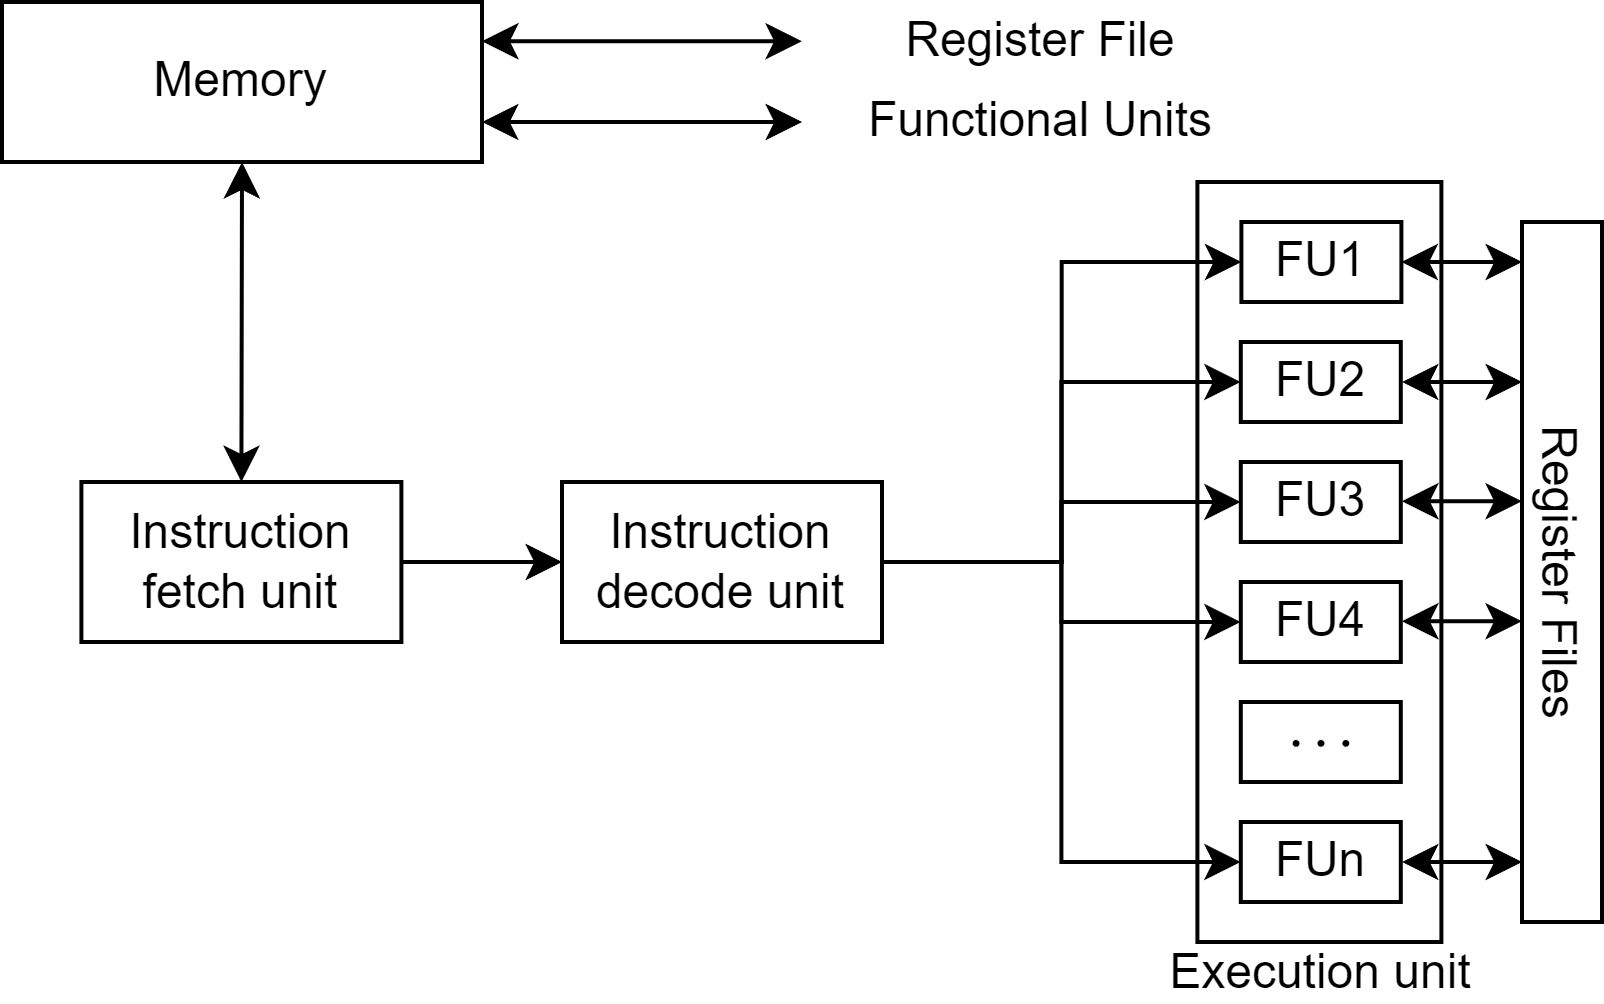
\includegraphics[width=0.75\linewidth]{images/vliw.png}
    \caption{VLIW machine configuration}
\end{figure}